\documentclass[12pt]{article}
\usepackage{amsmath}
\usepackage{amssymb}
\usepackage{tikz}

\begin{document}

The graph \( G_{\mathcal{F}} \) obtained from the formula \( \mathcal{F} = (X_1 \vee X_3) \wedge (X_2 \vee X_3 \vee X_5) \wedge (X_4 \vee X_5) \).

\begin{center}
    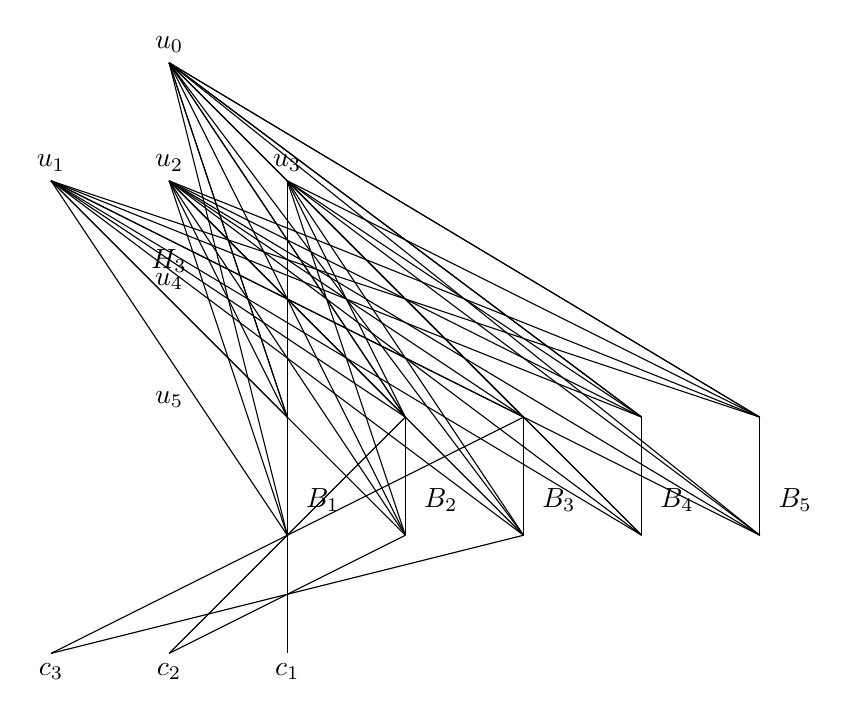
\begin{tikzpicture}[scale=1.5]
        
        % Define coordinates for the vertices in the top part of the graph
        \coordinate (u0) at (0, 0);
        \coordinate (u1) at (-1, -1);
        \coordinate (u2) at (0, -1);
        \coordinate (u3) at (1, -1);
        \coordinate (u4) at (0, -2);
        \coordinate (u5) at (0, -3);

        % Define coordinates for the vertices in the bottom part of the graph
        \foreach \x/\y [count=\i] in {1/-3, 2/-3, 3/-3, 4/-3, 5/-3}{
            \coordinate (b\x) at (\x, \y);
            \coordinate (a\x) at (\x, \y-1);
        }
        \coordinate (c1) at (1, -5);
        \coordinate (c2) at (0, -5);
        \coordinate (c3) at (-1, -5);

        % Draw edges between u_i and a_j
        \foreach \i in {0,1,2,3}{
            \foreach \j in {1,2,3,4,5}{
                \draw (u\i) -- (a\j);
            }
        }

        % Draw edges between u_i and b_j
        \foreach \i in {0,1,2,3}{
            \foreach \j in {1,2,3,4,5}{
                \draw (u\i) -- (b\j);
            }
        }

        % Draw edges between a_i and b_j
        \foreach \i in {1,2,3,4,5}{
            \draw (a\i) -- (b\i);
        }

        % Draw edges between a_i and c_j
        \foreach \i in {1,2,3}{
            \draw (a\i) -- (c\i);
        }

        % Draw edges between b_i and c_j
        \foreach \i in {1,2,3}{
            \draw (b\i) -- (c\i);
        }

        % Draw the central vertex and its connections
        \draw (u0) -- (b1);
        \draw (u0) -- (b2);
        \draw (u0) -- (b3);
        \draw (u0) -- (b4);
        \draw (u0) -- (b5);

        % Draw the subgraphs B_i
        \foreach \i in {1,2,3,4,5}{
            \draw (a\i) ++(0.3, 0.3) node {$B_\i$};
        }

        % Label the vertices in the top part of the graph
        \foreach \i/\j in {0/0, 1/1, 2/2, 3/3, 4/4, 5/5}{
            \node at (u\i) [above] {$u_\j$};
        }

        % Label the vertices in the bottom part of the graph
        \foreach \i in {1,2,3}{
            \node at (c\i) [below] {$c_\i$};
        }

        \node at (0, -1.5) [below] {$H_3$};

    \end{tikzpicture}
\end{center}

\end{document}